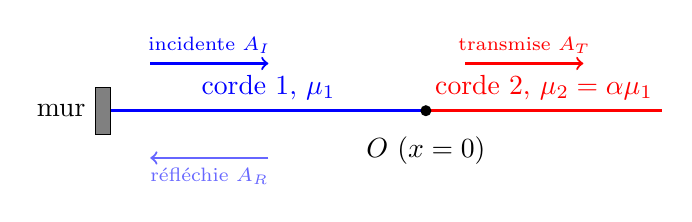
\begin{tikzpicture}[scale=1]
    \draw[fill=gray] (-4.2,-0.3) rectangle (-4,0.3);
    \draw[very thick, blue] (-4,0) -- (0,0) node[midway, above] {corde 1, $\mu_1$};
    \draw[very thick, red] (0,0) -- (3,0) node[midway, above] {corde 2, $\mu_2=\alpha\mu_1$};
    \fill (0,0) circle (2pt) node[below=6pt] {$O$ ($x=0$)};

    \draw[->, thick, blue] (-3.5,0.6) -- (-2,0.6) node[midway, above, font=\scriptsize] {incidente $A_I$};
    \draw[->, thick, blue!60] (-2,-0.6) -- (-3.5,-0.6) node[midway, below, font=\scriptsize] {réfléchie $A_R$};
    \draw[->, thick, red] (0.5,0.6) -- (2,0.6) node[midway, above, font=\scriptsize] {transmise $A_T$};

    \node[left] at (-4.2,0) {mur};
\end{tikzpicture}
